\chapter{Algorithms: Search}

\begin{enumerate}
    \item \textbf{uninformed search/ blind search}: The term means that the strategies have no additional information about states beyond that provided in the problem definition.\\
    All they can do is generate successors and distinguish a goal state from a non-goal state. 

    \item \textbf{ informed search or heuristic search}: Strategies that know whether one non-goal state is “more promising” than another\\
    The general approach we consider is called \textbf{best-first search}. (SEE: \fullref{Best-first Search})
\end{enumerate}

\section*{Notations}

\begin{customTableWrapper}{1.2}
\begin{longtable}{l p{8cm}}
    $b$ & branching factor; max number of children a parent node has\\

    $d$ & depth of the shallowest goal node\\

    $m$ & maximum length of any path in the state space\\

    $C$ & cost of solution\\

    $C^\ast$ & cost of optimal solution\\

    $l$ & predetermined depth limit \\

    $\epsilon$ & very small positive number (least step-cost)\\

    \hline

    $g(n)$ & lowest path cost to reach node $n$ from root node\\

    $f(n)$ & evaluation function \\

    $h(n)$ & heuristic function \\
\end{longtable}
\end{customTableWrapper}

\begin{enumerate}
    \item The evaluation function is construed as a cost estimate, so the node with the lowest evaluation is expanded first.

    \item $h(n)$ = estimated cost of the cheapest path from the state at node n to a goal state.\\
    $h(n)$ takes a node as input, but, unlike $g(n)$, it depends only on the state at that node.\\
    Heuristic functions are the most common form in which additional knowledge of the problem is imparted to the search algorithm.\\
    if $n$ is a goal node, then $h(n) = 0$
\end{enumerate}

\begin{customTableWrapper}{1.2}
\begin{longtable}{|l|p{4cm}|p{8cm}|}
    \hline
    \customTableHeaderColor
    \textbf{Function} & \textbf{Description} & \textbf{Purpose} \\ 
    \hline
    \endfirsthead
    
    \hline
    \endhead
    
    \hline
    \endfoot
    
    \hline
    \endlastfoot

    $g(n)$ & Lowest path cost to reach node $n$ from root & Represents the actual cost incurred to reach the node $n$ \\ \hline
    
    $f(n)$ & Evaluation function & Combines both $g(n)$ and $h(n)$ to estimate the total cost (typically $f(n) = g(n) + h(n)$) \\ \hline
    
    $h(n)$ & Heuristic function & Provides an estimate of the cost to reach the goal from node $n$ \\ \hline
    
\end{longtable}
\end{customTableWrapper}



\section{Linear Search Algorithm \cite{gfg-linear-search}}\label{Linear Search Algorithm}

\begin{table}[h]
    \begin{minipage}[t]{0.5\linewidth}
        \begin{figure}[H]
            \centering
            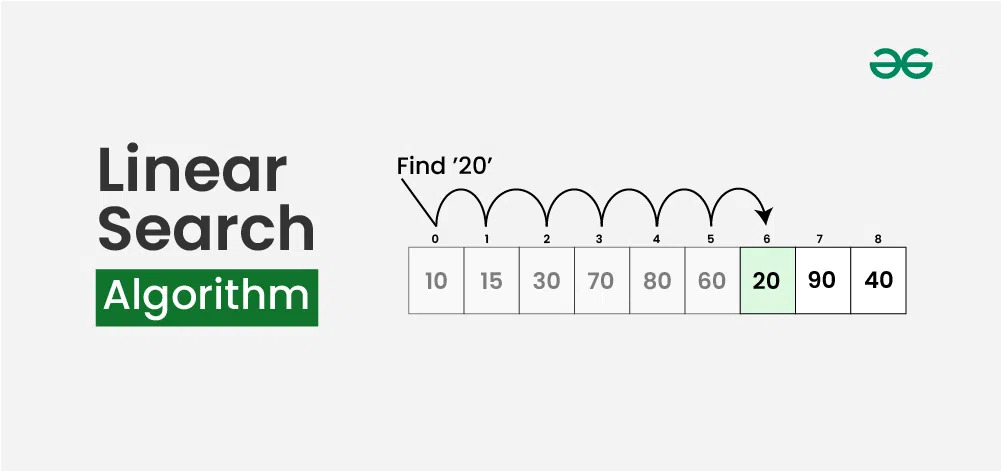
\includegraphics[width=\linewidth,height=6cm,keepaspectratio]{Pictures/ds-algo/Linear-Search-algorithm.jpg}
            \caption{Linear Search Algorithm}
        \end{figure}
    \end{minipage}
    \hfill
    \begin{minipage}[t]{0.35\linewidth}
        \begin{customTableWrapper}{1.2}
        \begin{table}[H]
            \begin{tabular}{l l l}
                \customTableHeaderColor
                \multicolumn{3}{c}{\textbf{Time Complexity}} \\
                 
                 Best Case & $O(1)$ & first index \\
                 Average Case & $O(N)$ &  \\
                 Worst Case & $O(N)$ & last index \\

                 \customTableHeaderColor
                 \multicolumn{3}{c}{\textbf{Space Complexity}}\\
                 
                 Auxiliary Space & $O(1)$ & iterator \\
            \end{tabular}
        \end{table}
        \end{customTableWrapper}
    \end{minipage}
\end{table}

\textbf{Steps}:
\begin{enumerate}
    \item \textbf{Start}: Begin at the first element of the collection of elements.
    \item \textbf{Compare}: Compare the current element with the desired element.
    \item \textbf{Found}: If the current element is equal to the desired element, return true or index to the current element.
    \item \textbf{Move}: Otherwise, move to the next element in the collection.
    \item \textbf{Repeat}: Repeat steps 2-4 until we have reached the end of collection.
    \item \textbf{Not found}: If the end of the collection is reached without finding the desired element, return that the desired element is not in the array.
\end{enumerate}

\begin{table}[h]
    \begin{minipage}[t]{0.48\linewidth}
        \textbf{Advantages}:
        \begin{enumerate}
            \item Linear search can be used irrespective of whether the array is sorted or not. 
            \item It can be used on arrays of any data type.
            \item Does not require any additional memory.
            \item It is a well-suited algorithm for small datasets.
        \end{enumerate}
    \end{minipage}
    \hfill
    \begin{minipage}[t]{0.48\linewidth}
        \textbf{Disadvantages}:
        \begin{enumerate}
            \item Linear search has a time complexity of $O(N)$, which in turn makes it \textbf{SLOW} for large datasets.
            \item \textbf{NOT} suitable for large arrays.
        \end{enumerate}
    \end{minipage}
\end{table}

\begin{lstlisting}[language=Python, caption=Linear Search Algorithm - Python]
def search(arr: list, N: int, x: object) -> int:
    for i in range(0, N):
        if (arr[i] == x):
            return i
    return -1
\end{lstlisting}

\section{Binary Search Algorithm \cite{gfg-binary-search}} \label{Binary Search Algorithm}

\begin{table}[H]
    \begin{minipage}[t]{0.45\linewidth}
        \begin{figure}[H]
            \centering
            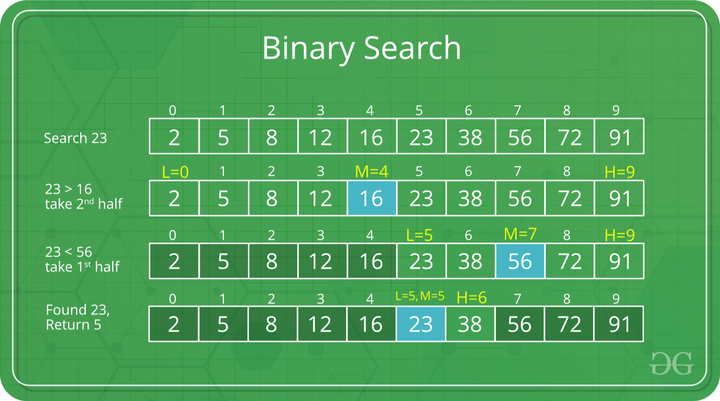
\includegraphics[width=\linewidth,height=6cm,keepaspectratio]{Pictures/ds-algo/BinarySearch.png}
            \caption{Binary Search Algorithm}
        \end{figure}
    \end{minipage}
    \hfill
    \begin{minipage}[t]{0.55\linewidth}
        \begin{customTableWrapper}{1.2}
        \begin{table}[H]
            \begin{tabular}{l l l}
                \customTableHeaderColor
                \multicolumn{3}{c}{\textbf{Time Complexity}} \\
                 
                 Best Case & $O(1)$ & \\
                 Average Case & $O(\log(N))$ &  \\
                 Worst Case & $O(\log(N))$ &  \\

                 \customTableHeaderColor
                 \multicolumn{3}{c}{\textbf{Space Complexity}}\\
                 
                 Auxiliary Space & $O(1)$ & \\
                 Auxiliary Space & $O(\log(N))$ & recursive call stack \\
            \end{tabular}
        \end{table}
        \end{customTableWrapper}
    \end{minipage}
\end{table}


\textbf{Steps}:
\begin{enumerate}
    \item Divide the search space into two halves by finding the middle index “mid”.
    \item Compare the middle element of the search space with the key.
    \item If the key is found at middle element, the process is terminated.
    \item If the key is not found at middle element, choose which half will be used as the next search space.
    \begin{enumerate}
        \item If the key is smaller than the middle element, then the left side is used for next search.
        \item If the key is larger than the middle element, then the right side is used for next search.
    \end{enumerate}
    \item This process is continued until the key is found or the total search space is exhausted.
\end{enumerate}

\begin{table}[h]
    \begin{minipage}[t]{0.48\linewidth}
        \textbf{Advantages}:
        \begin{enumerate}
            \item Binary search is faster than linear search, especially for large arrays.
            \item More efficient than other searching algorithms with a similar time complexity, such as interpolation search or exponential search.
            \item Binary search is well-suited for searching large datasets that are stored in external memory, such as on a hard drive or in the cloud.
        \end{enumerate}
    \end{minipage}
    \hfill
    \begin{minipage}[t]{0.48\linewidth}
        \textbf{Disadvantages}:
        \begin{enumerate}
            \item The array should be \textbf{sorted}.
            \item Binary search requires that the data structure being searched be stored in contiguous memory locations. 
            \item Binary search requires that the elements of the array be comparable, meaning that they must be able to be ordered.
        \end{enumerate}
    \end{minipage}
\end{table}

\begin{lstlisting}[language=Python, caption=Binary Search (iterative) - Python]
def binarySearch(arr: list, low: int, high: int, x: object) -> int:
    while low <= high:
        mid = low + (high - low) // 2

        # Check if x is present at mid
        if arr[mid] == x: return mid

        # If x is greater, ignore left half
        elif arr[mid] < x: low = mid + 1

        # If x is smaller, ignore right half
        else: high = mid - 1

    # If we reach here, then the element was not present
    return -1
\end{lstlisting}

\begin{lstlisting}[language=Python, caption=Binary Search (recursive) - Python]
def binarySearch(arr: list, low: int, high: int, x: object) -> int:
    # Check base case
    if high >= low:
        mid = low + (high - low) // 2
        
        # If element is present at the middle itself
        if arr[mid] == x: return mid
            
        # If element is smaller than mid, then it
        # can only be present in left subarray
        elif arr[mid] > x: 
            return binarySearch(arr, low, mid-1, x)

        # Else the element can only be 
        # present in right subarray
        else: return binarySearch(arr, mid + 1, high, x)

    # Element is not present in the array
    else: return -1
\end{lstlisting}

\section{Ternary Search \cite{gfg-ternary-search}}\label{Ternary Search}
\begin{table}[h]
    \begin{minipage}{0.5\linewidth}
        \begin{figure}[H]
            \centering
            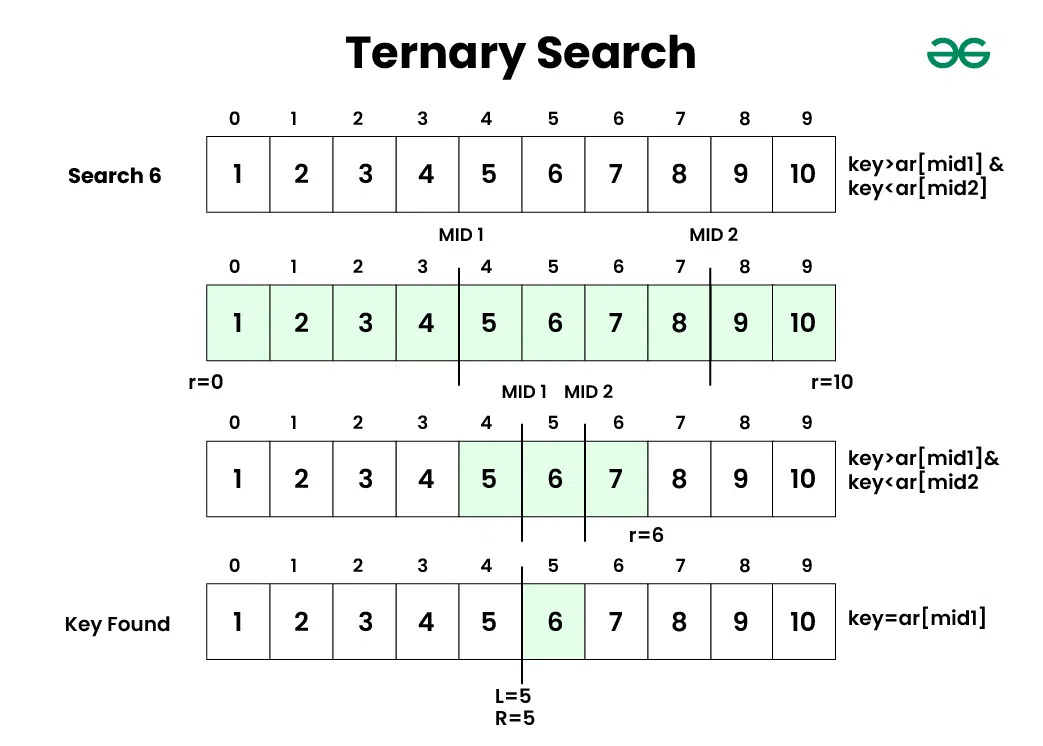
\includegraphics[width=\linewidth, height=10cm, keepaspectratio]{Pictures/ds-algo/Ternary-Search.jpg}
            \caption{Ternary Search}
        \end{figure}
    \end{minipage}
    \hfill
    \begin{minipage}{0.47\linewidth}
        \begin{customTableWrapper}{1.2}
        \begin{table}[H]
            \begin{tabular}{l l l}
                \customTableHeaderColor
                \multicolumn{3}{c}{\textbf{Time Complexity}} \\
                 
                 Recursive & $O(2*\log_3(N))$ & \\
                 Iterative & $O(\log_3(N))$ & \\

                 \customTableHeaderColor
                 \multicolumn{3}{c}{\textbf{Space Complexity}}\\
                 
                 Auxiliary Space & $O(2*\log_3(N))$ & Recursive \\
                 Auxiliary Space & $O(1)$ & Iterative \\
            \end{tabular}
        \end{table}
        \end{customTableWrapper}
    \end{minipage}
\end{table}

\vspace{0.2cm}
\textbf{Steps}:
\begin{enumerate}
    \item \textbf{Initialization}: Set two pointers, \textbf{left} and \textbf{right}, initially pointing to the first and last elements of our search space.

    \item \textbf{Divide the search space}:
    \begin{enumerate}
        \item Calculate two midpoints, mid1 and mid2, dividing the current search space into three roughly equal parts:
        \item[] $mid1 = left + (right - left) / 3$
        \item[] $mid2 = right - (right - left) / 3$
        \item The array is now effectively divided into $[left, mid1]$, $(mid1, mid2)$, and $[mid2, right]$.
    \end{enumerate}

    \item \textbf{Comparison with Target}:
    \begin{enumerate}
        \item If the \textbf{target} is equal to the element at \textbf{mid1} or \textbf{mid2}, the search is successful, and the index is returned.

        \item If the target is less than the element at mid1, update the right pointer to $mid1 - 1$.

        \item If the target is greater than the element at mid2, update the left pointer to $mid2 + 1$.

        \item If the target is between the elements at mid1 and mid2, update the left pointer to $mid1 + 1$ and the right pointer to $mid2 - 1$.
    \end{enumerate}

    \item \textbf{Repeat or Conclude}:
    \begin{enumerate}
        \item Repeat the process with the reduced search space until the target is found or the search space becomes empty.

        \item If the search space is empty and the target is not found, return a value indicating that the target is not present in the array.
    \end{enumerate}
\end{enumerate}

\begin{table}[h]
    \begin{minipage}[t]{0.48\linewidth}
        \textbf{Advantages}:
        \begin{enumerate}
            \item Ternary search can find maxima/minima for unimodal functions, where binary search is not applicable.
            
            \item Ternary Search has a time complexity of $O(2 * \log_3(N))$, which is more efficient than linear search and comparable to binary search.

            \item Fits well with optimization problems.
        \end{enumerate}
    \end{minipage}
    \hfill
    \begin{minipage}[t]{0.48\linewidth}
        \textbf{Disadvantages}:
        \begin{enumerate}
            \item Ternary Search is only applicable to ordered lists or arrays, and cannot be used on unordered or non-linear data sets.

            \item Ternary Search takes more time to find maxima/ minima of monotonic functions as compared to Binary Search.
        \end{enumerate}
    \end{minipage}
\end{table}

\begin{lstlisting}[language=Python, caption=Ternary Search (recursive) - Python]
def ternarySearch(l: int, r: int, key: int, ar: list) -> int:
    if (r >= l):
        # Find the mid1 and mid2
        mid1 = l + (r - l) //3
        mid2 = r - (r - l) //3

        # Check if key is present at any mid
        if (ar[mid1] == key):  return mid1
        
        if (ar[mid2] == key): return mid2
        
        # Since key is not present at mid,
        # check in which region it is present
        # then repeat the Search operation
        # in that region
        if (key < ar[mid1]): 
            # The key lies in between l and mid1
            return ternarySearch(l, mid1 - 1, key, ar)
        
        elif (key > ar[mid2]): 
            # The key lies in between mid2 and r
            return ternarySearch(mid2 + 1, r, key, ar)
        
        else: 
            # The key lies in between mid1 and mid2
            return ternarySearch(mid1 + 1, mid2 - 1, key, ar)
        
    # Key not found
    return -1
\end{lstlisting}
\begin{lstlisting}[language=Python, caption=Ternary Search (iterative) - Python]
def ternarySearch(l: int, r: int, key: int, ar: list) -> int:
    while r >= l:
        # Find mid1 and mid2
        mid1 = l + (r-l) // 3
        mid2 = r - (r-l) // 3

        # Check if key is at any mid
        if key == ar[mid1]: return mid1
        if key == ar[mid2]: return mid2

        # Since key is not present at mid, 
        # Check in which region it is present
        # Then repeat the search operation in that region
        if key < ar[mid1]:
            # key lies between l and mid1
            r = mid1 - 1
        elif key > ar[mid2]:
            # key lies between mid2 and r
            l = mid2 + 1
        else:
            # key lies between mid1 and mid2
            l = mid1 + 1
            r = mid2 - 1

    # key not found
    return -1
\end{lstlisting}


\section{Exponential Search \cite{gfg-exponential-search}}\label{Exponential Search}

\begin{customTableWrapper}{1.2}
\begin{table}[h]
    \begin{tabular}{l l l}
         \textbf{Time Complexity} & $O(\log(N))$ &  \\

         \customTableHeaderColor
         \multicolumn{3}{c}{\textbf{Space Complexity}}\\
         
         Auxiliary Space & $O(1)$ & iterative \\
         Auxiliary Space & $O(\log(N))$ & recursive \\
    \end{tabular}
\end{table}
\end{customTableWrapper}

\textbf{Steps}:
\begin{enumerate}
    \item Find range where element is present
    \item Do \fullref{Binary Search Algorithm} in above found range
\end{enumerate}

\begin{lstlisting}[language=Python, caption=Exponential Search - Python]
# Returns the position of first occurrence of x in array
def exponentialSearch(arr: list, n: int, x: object) -> int:
    # IF x is present at first 
    # location itself
    if arr[0] == x: return 0
         
    # Find range for binary search 
    # j by repeated doubling
    i = 1
    while i < n and arr[i] <= x: i = i * 2
     
    # Call binary search for the found range
    return binarySearch(arr, i // 2, min(i, n-1), x)
\end{lstlisting}


\section{Selective Search (CNN) \cite{https://www.geeksforgeeks.org/r-cnn-region-based-cnns/}}\label{Selective Search (CNN)}

\begin{table}[h]
    \begin{minipage}[t]{0.39\linewidth}
        \begin{figure}[H]
            \centering
            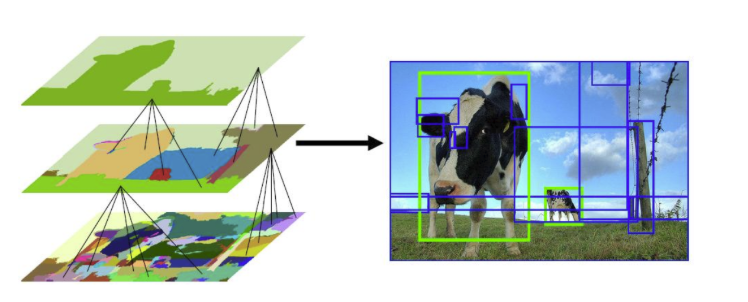
\includegraphics[width=\linewidth, height=3cm, keepaspectratio]{Pictures/convolutional-neural-network/rcnn-selective-search.png}
            \caption{Selective Search}
        \end{figure}        
    \end{minipage}
    \hfill
    \begin{minipage}[t]{0.59\linewidth}
        \begin{enumerate}
            \item Selective search is a \textbf{greedy algorithm} that combines smaller segmented regions to generate region proposals.
            
            \item This algorithm takes an image as input and output generates region proposals on it.
        
            \item This algorithm has the advantage over random proposal generation in that it limits the number of proposals to approximately 2000 and these region proposals have a high recall.
        \end{enumerate}    
    \end{minipage}
\end{table}


\vspace{0.2cm}
\textbf{Algorithm}:
\begin{enumerate}
    \item Generate initial sub-segmentation of the input image.

    \item Combine similar bounding boxes into larger ones recursively.

    \item Use these larger boxes to generate region proposals for object detection.
\end{enumerate}

\vspace{0.2cm}
\textbf{Challenges}:
\begin{enumerate}
    \item The selective Search algorithm is very rigid and there is no learning happening in that. This sometimes leads to bad region proposal generation for object detection.
\end{enumerate}





\section{Tree Search (generic) \cite{aci-1}}\label{Tree Search (generic)}

\begin{algorithm}[H]
    \caption{An informal description of the general tree-search algorithm.}

    \SetKwFunction{FUNCTION}{TREE-SEARCH}
    \SetKwProg{Fn}{function}{:}{}
    \Fn{\FUNCTION{problem}}{
        initialize the frontier using the initial state of problem\\
        \SetKwBlock{Loop}{Loop do}{}
        \Loop{
            \If{frontier is empty}{
                \Return failure
            }
            choose a leaf node and remove it from the frontier\\
            \If{node contains a goal state}{
                 \Return corresponding solution
            }
            expand the chosen node, adding the resulting nodes to the frontier
        }
    }
\end{algorithm}





\section{Graph Search (generic) \cite{aci-1}}\label{Graph Search (generic)}

\begin{algorithm}[H]
    \caption{An informal description of the general graph-search algorithm.}

    \SetKwFunction{FUNCTION}{GRAPH-SEARCH}
    \SetKwProg{Fn}{function}{:}{}
    \Fn{\FUNCTION{problem}}{
        initialize the frontier using the initial state of problem\\
        \textbf{initialize the explored set to be empty}\\
        \SetKwBlock{Loop}{Loop do}{}
        \Loop{
            \If{frontier is empty}{
                \Return failure
            }
            choose a leaf node and remove it from the frontier\\
            \If{node contains a goal state}{
                 \Return corresponding solution
            }
            \textbf{add the node to the explored set}\\
            expand the chosen node, adding the resulting nodes to the frontier\\
            \hspace{0.4cm} \textbf{only if not in the frontier or explored set}
        }
    }
\end{algorithm}


\section{Breadth-first search (BFS) \cite{aci-1}}\label{Breadth-first search BFS}

\begin{center}
    $f(n) = g(n)$
\end{center}

\begin{enumerate}
    \item Breadth-first search is a simple strategy in which the root node is expanded first, then all the successors of the root node are expanded next, then their successors, and so on. 
    
    \item In general, all the nodes are expanded at a given depth in the search tree before any nodes at the next level are expanded.

    \item shallowest unexpanded node is chosen for expansion

    \item There is one slight tweak on the general graph-search algorithm, which is that the goal test is applied to each node when it is generated rather than when it is selected for expansion.

    \item  the memory requirements are a bigger problem for breadth-first search than is the execution time.

    \item nodes in the explored set: $\mathcal{O}(b^{d-1})$

    \item nodes in the frontier: $\mathcal{O}(b^{d})$
\end{enumerate}


\begin{customTableWrapper}{1.2}
\begin{longtable}{p{4cm} p{8cm}}
    Space Complexity & $\mathcal{O}(b^d)$ \\

    Time Complexity & $\mathcal{O}(b^d)$ \\

    \hline
    
    Completeness & YES \textbf{if} \textit{b \& d are finite} \textbf{else} NO\\

    Optimal & YES \textbf{if} \textit{all steps cost same} \textbf{else} NO \\

    Can Handle infinite state space? & NO \\
\end{longtable}
\end{customTableWrapper}


\begin{algorithm}[H]
\caption{Breadth-first search on a graph.}

\SetKwFunction{FUNCTION}{BREADTH-FIRST-SEARCH}
\SetKwProg{Fn}{function}{:}{}
\Fn{\FUNCTION{problem}}{
    node $\gets$ a node with STATE = \textit{problem}.INITIAL-STATE, PATH-COST = 0\\

    \If{\textit{problem}.GOAL-TEST(\textit{node}.STATE)}{
         \Return SOLUTION(\textit{node})
    }

    frontier $\gets$ a FIFO queue with node as the only element\\

    explored $\gets$ an empty set\\
    
    \SetKwBlock{Loop}{Loop do}{}
    \Loop{
        \If{EMPTY?(\textit{frontier})}{
            \Return failure
        }

        \Comment{chooses the shallowest node in frontier}
        node $\gets$ POP(\textit{frontier}) \\

        add \textit{node}.STATE to \textit{explored}\\

        \For{\textbf{each} action \textbf{in} problem.ACTIONS(node.STATE)}{
            \textit{child} $\gets$ CHILD-NODE(\textit{problem, node, action})\\
            
            \If{\textit{child}.STATE is not in \textit{explored} or \textit{frontier}}{
                \If{\textit{problem}.GOAL-TEST(\textit{child}.STATE)}{
                    \Return SOLUTION(\textit{child})
                }
                
                \textit{frontier} $\gets$ INSERT(\textit{child, frontier})
            }
        }
    }
}
\end{algorithm}




\section{Uniform-cost search (UCS) \cite{aci-1}}\label{Uniform-cost search (UCS)}

\begin{center}
    $f(n) = g(n)$
\end{center}

\begin{enumerate}
    \item algorithm that is optimal with any step-cost function

    \item Instead of expanding the shallowest node, uniform-cost search expands the node $n$ with the lowest path cost $g(n)$.

    \item stores the frontier as a \textbf{priority queue} ordered by $g$

    \item goal test is applied to a node when it is selected for expansion rather than when it is first generated\\
    first goal node that is generated may be on a sub-optimal path

    \item a test is added in case a better path is found to a node currently on the frontier

    \item uniform-cost search expands nodes in order of their optimal path cost

    \item Uniform-cost search does not care about the number of steps a path has, but only about their total cost.
\end{enumerate}

\vspace{0.5cm}

\begin{customTableWrapper}{1.2}
\begin{longtable}{p{3cm} p{6cm}}
    Space Complexity & $\mathcal{O}(b^{1 + \dfloor {C^\ast/ \epsilon}})$ \\

    Time Complexity & $\mathcal{O}(b^{1 + \dfloor {C^\ast/ \epsilon}})$ \\

    \hline
    
    Completeness & YES \textbf{if} \textit{b \& d are finite \textbf{and} $\epsilon > 0$} \textbf{else} NO\\

    Optimal & YES \\

    Can Handle infinite state space? & NO \\
\end{longtable}
\end{customTableWrapper}


\begin{algorithm}[H]
\caption{Uniform-cost search on a graph}

\SetKwFunction{FUNCTION}{UNIFORM-COST-SEARCH}
\SetKwProg{Fn}{function}{:}{}
\Fn{\FUNCTION{problem}}{
    \textit{node} $\gets$ a node with STATE = \textit{problem}.INITIAL-STATE, PATH-COST = 0\\
    
    \textit{frontier} $\gets$ a priority queue ordered by PATH-COST, with \textit{node} as the only element \\
    
    \textit{explored} $\gets$ an empty set\\

    \SetKwBlock{Loop}{Loop do}{}
    \Loop{
        \If{EMPTY?(\textit{frontier})}{
            \Return failure
        }
        \Comment{chooses the lowest-cost node in frontier}
        \textit{node} $\gets$ POP(\textit{frontier}) \\

        \If{\textit{problem}.GOAL-TEST(\textit{node}.STATE)}{
            \Return SOLUTION(\textit{node})
        }

        add \textit{node}.STATE to explored\\

        \For{\textbf{each} action \textbf{in} problem.ACTIONS(node.STATE)}{
            \textit{child} $\gets$ CHILD-NODE(\textit{problem,node,action})\\
            
            \If{child.STATE \textbf{is not in} explored \textbf{or} frontier}{
                \textit{frontier} $\gets$ INSERT(\textit{child, frontier})
            }
            \ElseIf{child.STATE \textbf{is in} frontier with higher PATH-COST}{
                replace that frontier node with child
            }
        }
    }
}
\end{algorithm}



\section{Depth-first search (DFS) \cite{aci-1}} \label{Depth-first search (DFS)}

\begin{center}
    $f(n) = g(n)$
\end{center}

\begin{enumerate}
    \item Depth-first search always expands the deepest node in the current frontier of the search tree.

    \item The search proceeds immediately to the deepest level of the search tree, where the nodes have no successors.\\
    As those nodes are expanded, they are dropped from the frontier, so then the search “backs up” to the next deepest node that still has unexplored successors.

    \item The graph-search version, which avoids repeated states and redundant paths, is complete in finite state spaces because it will eventually expand every node.\\
    The tree-search version, on the other hand, is not complete

    \item A variant of depth-first search called \textbf{backtracking search} uses still less memory.\\
    In backtracking, \textbf{only one successor} is generated at a time rather than all successors; each \textbf{partially expanded} node remembers which successor to generate next.\\
    In this way, only $\mathcal{O}(m)$ memory is needed rather than $\mathcal{O}(bm)$.
\end{enumerate}


\begin{customTableWrapper}{1.2}
\begin{longtable}{p{3cm} p{6cm}}
    Space Complexity & $\mathcal{O}(bm)$ \\

    Time Complexity & $\mathcal{O}(b^m)$ \\

    \hline

    Completeness & YES \textbf{if} \textit{b \& d are finite \textbf{and} algorithm = GRAPH-SEARCH} \textbf{else} NO\\

    Optimal & NO \\

    Can Handle infinite state space? & NO \\
\end{longtable}
\end{customTableWrapper}


\section{Depth-limited search (DLS) \cite{aci-1}} \label{Depth-limited search (DLS)}

\begin{center}
    $f(n) = g(n)$
\end{center}

\begin{enumerate}
    \item The failure of depth-first search in infinite state spaces can be alleviated by supplying depth-first search with a \textbf{predetermined depth limit} $l$.
    
    \item Nodes at depth $l$ are treated as if they have no successors. 
    
    \item The depth limit solves the infinite-path problem. 
    
    \item Unfortunately, it also introduces an additional source of incompleteness if we choose $l < d$, that is, the shallowest goal is beyond the depth limit. (This is likely when d is unknown.) 
    
    \item Depth-limited search will also be non-optimal if we choose $l > d$.
\end{enumerate}


\begin{customTableWrapper}{1.2}
\begin{longtable}{p{3cm} p{6cm}}
    Space Complexity & $\mathcal{O}(bl)$ \\

    Time Complexity & $\mathcal{O}(b^l)$ \\

    \hline

    Completeness & YES \textbf{if} \textit{$l \geq d$} \textbf{else} NO \\

    Optimal & NO \\

    Can Handle infinite state space? & YES \\
\end{longtable}
\end{customTableWrapper}


\begin{algorithm}[H]
\caption{A recursive implementation of depth-limited tree search.}

\SetKwFunction{FUNCTION}{DEPTH-LIMITED-SEARCH}
\SetKwProg{Fn}{function}{:}{}
\Fn{\FUNCTION{problem, limit}}{
    \Return RECURSIVE-DLS(MAKE-NODE(\textit{problem}.INITIAL-STATE), \textit{problem, limit})
}

\SetKwFunction{FUNCTION}{RECURSIVE-DLS}
\SetKwProg{Fn}{function}{:}{}
\Fn{\FUNCTION{node, problem, limit}}{
    \If{problem.GOAL-TEST(\textit{node}.STATE) }{
        \Return SOLUTION(\textit{node})
    }
    \ElseIf{limit = 0}{
        \Return cutoff
    }
    \Else{
        \textit{cutoff\_occurred?} $\gets$ false \\

        \For{\textbf{each} action \textbf{in} \textit{problem}.ACTIONS(\textit{node}.STATE)}{
            \textit{child} $\gets$ CHILD-NODE(\textit{problem, node, action})\\

            result $\gets$ RECURSIVE-DLS(\textit{child, problem, limit - 1})\\

            \If{result = cutoff}{
                \textit{cutoff\_occurred?} $\gets$ true
            }
            \ElseIf{result $\neq$ failure}{
                \Return result
            }
        }
        \If{cutoff\_occurred?}{
            \Return cutoff
        }
        \Else{
            \Return failture
        }
    }
}
\end{algorithm}


\section{Iterative deepening depth-first search/ Iterative deepening search (IDS) \cite{aci-1}} \label{Iterative deepening depth-first search/ Iterative deepening search (IDS)}

\begin{center}
    $f(n) = g(n)$
\end{center}

\begin{enumerate}
    \item Iterative deepening search (or iterative deepening depth-first search) is a general strategy, often used in combination with depth-first tree search, that finds the best depth limit. 
    
    \item It does this by gradually increasing the limit - first 0, then 1, then 2, and so on - until a goal is found.
    
    \item This will occur when the depth limit reaches d, the depth of the shallowest goal node.

    \item iterative deepening is the preferred uninformed search method when the search space is large and the depth of the solution is not known.
\end{enumerate}

\vspace{0.5cm}

\begin{customTableWrapper}{1.2}
\begin{longtable}{p{3cm} p{6cm}}
    Space Complexity & $\mathcal{O}(bd)$ \\

    Time Complexity & $\mathcal{O}(b^d)$ \\

    \hline

    Completeness & YES \textbf{if} \textit{finite} \textbf{else} NO \\

    Optimal & YES \textbf{if} \textit{all path costs same} \textbf{else} NO \\

    Can Handle infinite state space? & YES \\
\end{longtable}
\end{customTableWrapper}

\begin{algorithm}[H]
\caption{The iterative deepening search algorithm, which repeatedly applies depth-limited search with increasing limits. It terminates when a solution is found or if the depth-limited search returns failure, meaning that no solution exists.}

\SetKwFunction{FUNCTION}{ITERATIVE-DEEPENING-SEARCH}
\SetKwProg{Fn}{function}{:}{}
\Fn{\FUNCTION{problem}}{
    \For{depth = $0$ \textbf{to} $\infty$}{
        \textit{result} $\gets$ DEPTH-LIMITED-SEARCH(problem,depth)\\

        \If{result $\neq$ cutoff}{
            \Return result
        }
    }
}
\end{algorithm}




\section{Iterative Lengthening Search (ILS) \cite{aci-1}} \label{Iterative Lengthening Search (ILS)}

\begin{center}
    $f(n) = g(n)$
\end{center}

\begin{enumerate}
    \item The idea is to use increasing path-cost limits instead of increasing depth limits.

    \item uses \fullref{Depth-limited search (DLS)} version of \fullref{Uniform-cost search (UCS)}
\end{enumerate}


\section{Bidirectional search \cite{aci-1}} \label{Bidirectional search}

\begin{enumerate}
    \item The idea behind bidirectional search is to run two simultaneous searches - one forward from the initial state and the other backward from the goal - hoping that the two searches meet in the middle.

    \item Bidirectional search is implemented by replacing the goal test with a check to see whether the frontiers of the two searches intersect; if they do, a solution has been found.

    \item first such solution found may not be optimal, even if the two searches are both breadth-first; some additional search is required to make sure there isn’t another short-cut across the gap.

    \item The check can be done when each node is generated or selected for expansion and, with a hash table, will take constant time.

    \item Let the predecessors of a state x be all those states that have x as a successor.\\
    Bidirectional search requires a method for computing predecessors.\\
    When all the actions in the state space are reversible, the predecessors of x are just its successors.

    \item  if the goal is an abstract description, such as the goal that “no queen attacks another queen” in the n-queens problem, then bidirectional search is difficult to use.
\end{enumerate}

\begin{customTableWrapper}{1.2}
\begin{longtable}{p{3cm} p{6cm}}
    Space Complexity & $\mathcal{O}(b^{d/2})$ \\

    Time Complexity & $\mathcal{O}(b^{d/2})$ \\

    \hline

    Completeness & YES \textbf{if} \textit{finite} \textbf{else} NO \\

    Optimal & YES \textbf{if} \textit{additional search is done} \textbf{else} NO \\

    Can Handle infinite state space? & NO \\
\end{longtable}
\end{customTableWrapper}



\section{Best-first Search \cite{aci-1}} \label{Best-first Search}

\begin{enumerate}
    \item Best-first search is an instance of the general TREE-SEARCH or GRAPH-SEARCH algorithm in which a node is selected for expansion based on an evaluation function, $f(n)$.
\end{enumerate}


\section{Greedy best-first search (GBFS) \cite{aci-1}} \label{Greedy best-first search (GBFS)}

\begin{center}
    $f(n) = h(n)$
\end{center}

\begin{enumerate}
    \item Greedy best-first search8 tries to expand the node that is closest to the goal, on the grounds that this is likely to lead to a solution quickly.

    \item With a good heuristic function, however, the complexity can be reduced substantially. 
    
    \item The amount of the reduction depends on the particular problem and on the quality of the heuristic.
\end{enumerate}

\begin{customTableWrapper}{1.2}
\begin{longtable}{p{3cm} p{6cm}}
    Space Complexity & $\mathcal{O}(b^m)$ \\

    Time Complexity & $\mathcal{O}(b^m)$ \\

    \hline

    Completeness & YES \textbf{if} \textit{graph algo} \textbf{else} NO \\

    Optimal & NO \\

    Can Handle infinite state space? & NO (even in finite space) \\
\end{longtable}
\end{customTableWrapper}




\section{A* (A-star) search \cite{aci-1}} \label{A* (A-star) search}

\begin{center}
    $f(n) = g(n) + h(n)$
\end{center}


\begin{enumerate}
    \item Since $g(n)$ gives the path cost from the start node to node $n$, and $h(n)$ is the estimated cost of the cheapest path from $n$ to the goal, we have \\
    $f(n)$ = estimated cost of the cheapest solution through $n$

    \item The algorithm is identical to \verb|UNIFORM-COST-SEARCH| except that A* uses $g + h$ instead of $g$.

    
\end{enumerate}


\begin{customTableWrapper}{1.2}
\begin{longtable}{p{3cm} p{6cm}}
    Space Complexity & $\mathcal{O}()$ \\

    Time Complexity & $\mathcal{O}()$ \\

    \hline

    Completeness &  YES  \\

    Optimal & YES \\

    Consistent solution & YES \textbf{if} $h(n) \leq c(n, a, n') + h(n')$ \textbf{else} NO \\

    Can Handle infinite state space? &  \\

\end{longtable}
\end{customTableWrapper}

\subsection{Conditions for optimality: Admissibility and consistency \cite{aci-1}}

\begin{enumerate}
    \item condition we require for optimality is that $h(n)$ be an admissible heuristic.

    \item An \textbf{admissible heuristic}\indexlabel{admissible heuristic} is one that \textit{never overestimates} the cost to reach the goal.
    
    \item Because $g(n)$ is the actual cost to reach $n$ along the current path, and $f(n) = g(n) + h(n)$, we have as an immediate consequence that $f(n)$ never overestimates the true cost of a solution along the current path through $n$.

    \item Admissible heuristics are by nature optimistic because they think the cost of solving the problem is less than it actually is.

    \item Straight-line distance is admissible because the shortest path between any two points is a straight line, so the straight line cannot be an overestimate.

    \item slightly stronger condition called \textbf{consistency} (or sometimes \textbf{monotonicity}) is required only for applications of A* to graph search.

    \item A heuristic $h(n)$ is consistent if, for every node $n$ and every successor $n'$ of $n$ generated by any action $a$, the estimated cost of reaching the goal from $n$ is no greater than the step cost of getting to $n'$ plus the estimated cost of reaching the goal from $n'$

    \item This is a form of the general triangle inequality, which stipulates that each side of a triangle cannot be longer than the sum of the other two sides.\\
    Here, the triangle is formed by $n$, $n'$, and the goal $G_n$ closest to $n$. 

    \item For an admissible heuristic, the inequality makes perfect sense: if there were a route from n to $G_n$ via $n'$ that was cheaper than $h(n)$, that would violate the property that $h(n)$ is a lower bound on the cost to reach $G_n$.
\end{enumerate}

\subsection{Optimality of A* \cite{aci-1}}

\begin{enumerate}
    \item the tree-search version of A* is optimal if $h(n)$ is admissible

    \item graph-search version is optimal if $h(n)$ is consistent

    \item if $h(n)$ is consistent, then the values of $f(n)$ along any path are non-decreasing.

    \item whenever A* selects $a$ node $n$ for expansion, the optimal path to that node has been found

    \item If C* is the cost of the optimal solution path, then we can say the following:
    \begin{enumerate}
        \item A* expands all nodes with $f(n) < C*$

        \item A* might then expand some of the nodes right on the “goal contour” (where $f(n) = C*$) before selecting a goal node.
    \end{enumerate}

    \item among optimal algorithms of this type - algorithms that extend search paths from the root and use the same heuristic information - A* is \textbf{optimally efficient} for any given consistent heuristic.

    \item no other optimal algorithm is guaranteed to expand fewer nodes than A* (except possibly through tie-breaking among nodes with $f(n)$ = C*). 
    
    \item any algorithm that does not expand all nodes with $f(n)$ < C* runs the risk of missing the optimal solution.

    \item 
\end{enumerate}
















